% Systemmodell
\section{Systemmodell}
Die Anwendung ist nach dem Prinzip des \gls{MVC}-Entwurfmusters aufgebaut. Das folgende Diagramm zeigt, wie die Software gegliedert ist.
Durch die Verwendung von \gls{MVC} wird die Architektur strukturierter und Modifikationen am Programm werden vereinfacht. 
\\
\begin{figure}
    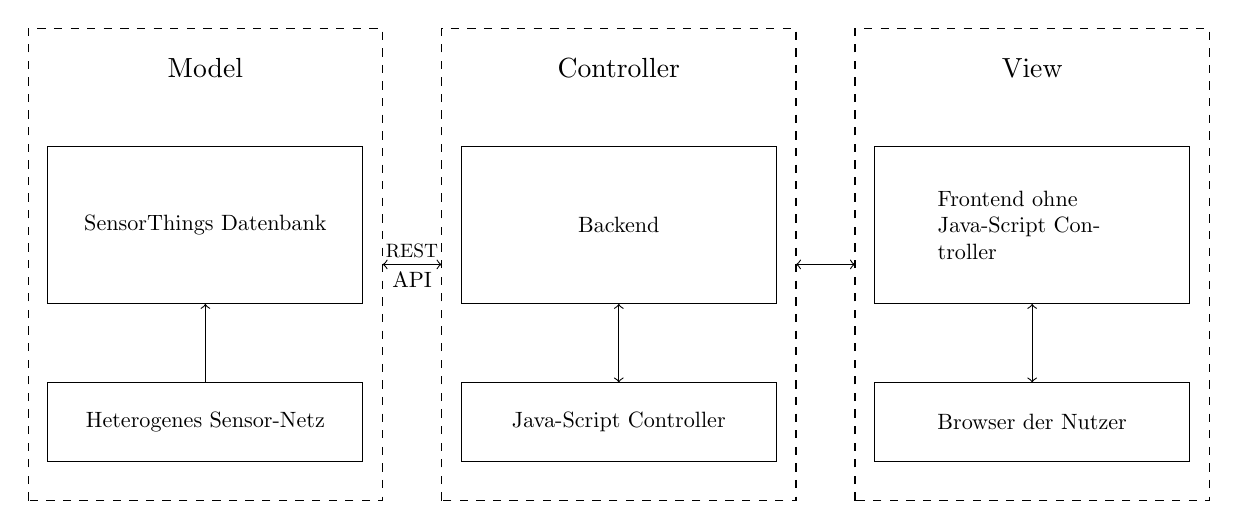
\begin{tikzpicture}[node distance=2cm]

        %Model
        \begin{scope}[shift={(0,0)},local bounding box=M]
            \draw (0,0) [dashed] rectangle (4.5,6);
            \node[scale=1] at (2.25,5.5) {Model};
            \begin{scope}[local bounding box=Datenbank]
                \draw (0.25,2.5) rectangle (4.25,4.5);
                \node[scale=0.8] at (2.25,3.5) {SensorThings Datenbank};
            \end{scope}
            \begin{scope}[local bounding box=Sensoren]
                \draw (0.25,0.5) rectangle (4.25,1.5);
                \node[scale=0.8] at (2.25,1) {Heterogenes Sensor-Netz};
            \end{scope}
        \end{scope}
        
        %Controller
        \begin{scope}[shift={(5.25,0)},local bounding box=C]
            \draw (0,0) [dashed] rectangle (4.5,6);
            \node[scale=1] at (2.25,5.5) {Controller};
            \begin{scope}[local bounding box=Backend]
                \draw (0.25,2.5) rectangle (4.25,4.5);
                \node[scale=0.8] at (2.25,3.5) {\softwarename Backend};
            \end{scope}
            \begin{scope}[local bounding box=User-Backend]
                \draw (0.25,0.5) rectangle (4.25,1.5);
                \node[scale=0.8] at (2.25,1) {Java-Script Controller};
            \end{scope}
        \end{scope}

        %View
        \begin{scope}[shift={(10.5,0)},local bounding box=V]
            \draw (0,0) [dashed] rectangle (4.5,6);
            \node[scale=1] at (2.25,5.5) {View};

            \begin{scope}[local bounding box=Frontend]
                \draw (0.25,2.5) rectangle (4.25,4.5);
                \node[scale=0.8,text width=3cm] at (2.25,3.5) {\softwarename Frontend ohne Java-Script Controller};
            \end{scope}
            \begin{scope}[local bounding box=Browser]
                \draw (0.25,0.5) rectangle (4.25,1.5);
                \node[scale=0.8] at (2.25,1) {Browser der Nutzer};
            \end{scope}
        \end{scope}

            
        \draw[<->] (M.east) -- (C.west) node[midway,above,scale=0.7] {REST} node[midway,below,scale=0.8] {API};
        \draw[<->] (C.east) -- (V.west);
        \draw[<-] (Datenbank.south) -- (Sensoren.north);
        \draw[<->] (Frontend.south) -- (Browser.north);
        \draw[<->] (Backend.south) -- (User-Backend.north);

    \end{tikzpicture}
    \caption{Diagramm des System-Aufbaus}
\end{figure}
\\
\begin{itemize}
    \item \textbf{Model:} Im Model findet die Datenhaltung statt. Alle durch die Sensoren gesammelten Daten werden in der Datenbank nach dem Standard der \gls{SensorThings API} gespeichert. Die Datenhaltung wird in \softwarename nicht implementiert.
        Zum Controller hin ist das Model über die \gls{RESTAPI} angebunden.
    \item \textbf{Controller:} Der Controller bereitet die Daten für die Darstellung auf und führt Operationen aus.
        Das \softwarename Backend lädt und speichert die Daten der \glspl{Sensor} aus der Datenbank zwischen. Das Backend sorgt somit auch dafür, dass die Nutzer bei der Anzeige der Daten nicht lange auf die Datenbank warten müssen, sondern die Daten schnellstmöglich gezeigt bekommen.
        Das \softwarename Backend läuft auf dem Webserver. Auf der Seite des Nutzers kommunizieren einige clientseitige \gls{JavaScript} Controller mit dem Backend.
    \item \textbf{View:} Die View organisiert die Anzeige der Daten für den Nutzer.
        Das \softwarename Frontend läuft auf dem Webserver und berechnet in Abstimmung mit dem Controller die angezeigten Daten.
        Im Browser des Nutzers werden die Daten schlussendlich angezeigt.
\end{itemize}
